\documentclass[DM,authoryear,toc]{lsstdoc}
% lsstdoc documentation: https://lsst-texmf.lsst.io/lsstdoc.html
\input{meta}

% Package imports go here.

% Local commands go here.

%If you want glossaries
%\input{aglossary.tex}
%\makeglossaries

\title{Lunar Complications in the Scheduling of Deep Drilling Fields}

% Optional subtitle
% \setDocSubtitle{A subtitle}

\author{%
Eric~Neilsen, Lynne~Jones, and Peter~Yoachim
}

\setDocRef{RTN-014}
\setDocUpstreamLocation{\url{https://github.com/lsst/rtn-014}}

\date{\vcsDate}

% Optional: name of the document's curator
% \setDocCurator{The Curator of this Document}

\setDocAbstract{%
The cadence of measurements of objects in Legacy Survey of Space and Time (LSST) Deep Drilling Fields (DDFs) does not match the observing cadence for all objects, because objects detected in one sequence of exposures may be too faint to be detected in others: even when fields are observed at an optimum time within each night, the limiting magnitude can vary by more than 2 magnitudes over a lunation.
This note examines the effects of the variation in sky brightness due to the moon on the cadence of measurements of objects in Legacy Survey of Space and Time (LSST) Deep Drilling Fields (DDFs).
Plots of the variation in limiting magnitude by night are shown for each DDF, and physical explanations for its major characteristics discussed.
A few strategies for minimizing the impact are described, trade-offs highlighted, and a list of related questions on science requirements raised.
}

% Change history defined here.
% Order: oldest first.
% Fields: VERSION, DATE, DESCRIPTION, OWNER NAME.
% See LPM-51 for version number policy.
\setDocChangeRecord{%
  \addtohist{1}{YYYY-MM-DD}{Unreleased.}{Eric Neilsen}
}


\begin{document}

% Create the title page.
\maketitle
% Frequently for a technote we do not want a title page  uncomment this to remove the title page and changelog.
% use \mkshorttitle to remove the extra pages

% ADD CONTENT HERE
% You can also use the \input command to include several content files.

\section{Summary}

\begin{enumerate}
\item Several important science uses for Deep Drilling Fields (DDFs) require detections of objects on a cadence without long gaps.
  The roughly monthly lunar cycle presents special problems for achieving this, for two reasons:
\begin{itemize}
\item The filter changer on the telescope cannot hold all filters at the same time.
  To allow observing using all filters, there must be periods of time during which at least one filter is not available for use.
\item Even if all filters were available, and each field were observed at the best possible time each night, sky brightness due to scattered moonlight in bright time would prevent detection of a substantial number of objects detected during dark time.
  In most fields, the limiting magnitude in g at full moon is 2 magnitudes brighter than in dark time, when observed at the optimal time during each night.
  To achieve a uniform depth on all nights on which a DDF is observed, the exposure times would need to be 40 times longer (in g) in bright time than dark time.
  In other filters, the difference is less extreme, but still substantial.
\end{itemize}
\item Each lunation, there are two important dates for understanding bright time gaps: the date of full moon, and the date on which the moon is closest to the DDF pointing.
\begin{itemize}
\item Exposures using any filter are affected by both, but the relative importance varies with wavelength: proximity to the moon is more important for longer wavelength light, while lunar phase is more important for shorter.
\item For a given field, at the start of an observing season the full moon occurs about a week before the date of the smallest angle between the field and the moon.
  In the center of the season, full moon and the date of smallest angle occur on the same night. Late in the season, full moon occurs about a week after the date of smallest angle.
\item At the center of an observing season, when the full moon coincides with the date of smallest angle, the depth of the field at the worst night of the lunation is most severely affected, but the number of nights over which the depths of a field is compromised is minimized: in the center of the season, sky brightness induced cadence gaps affect the most objects, but the duration of these gaps is at a minimum.
  For example, in the COSMOS field in g, the bright time at the center of the season creates gaps for objects more than 2 magnitudes brighter than the dark sky limiting magnitude, but the duration of this gap is only four nights.
\item At the edges of the seasons, the sky brightness of the brightest nights is less, but the duration of gaps is longer.
  Repeating the example of the COSMOS field in g, objects 2 magnitudes brighter than the dark sky limiting magnitude can be observed throughout the bright time (and so have an uninterrupted cadence), while objects 1.5 magnitudes brighter suffer a 9 night gap, and those one magnitude brighter suffer a 12 night gap.
\end{itemize}
\item Many of the DDFs have similar Right Ascensions, and so have overlapping seasons: different DDFs compete with each other for time. When the moon is waxing (the start of each bright time), if there is any dark or gray time in the night (during which the moon is near or below the horizon), it is at the end of the night.
  When the moon is waning, if there is any dark or gray time, it is at the start of the night. To minimize the length of the disruption in cadence (for objects within 1.5 to 2 magnitudes of the dark time limiting magnitude), a field needs to be observed in this window at the start and end of each bright time.
  However, all fields at similar R.A. compete for this same window of time. A strategy for prioritizing the use of this time among different fields is therefore required.
\item Weather effects complicate the minimization of gaps around bright time.
  The bright time gap at a given limiting magnitude is minimized if the field is observed on the last night before a sequence of nights in will fall beneath the detection threshold.
  If the field is not to be observed on consecutive nights, then it would not be scheduled on the 2nd night before this bright time gap.
  This poses a risk: if the weather is poor on the last night before the bright time gap, then the gap will be at least one night longer than necessary.
\end{enumerate}

\section{Introduction}

One of the primary ``mini-surveys'' of the Vera C. Rubin Observatory Legacy Survey of Space and Time (LSST) is the Deep Drilling Field (DDF) survey. Fields in the DDF survey will be scheduled to attain greater photometric depth and more frequent temporal sampling than the primary ``Wide Fast Deep'' (WFD) survey.
The frequent temporal sampling is valuable for measuring well sampled light curves for sources that vary on timescales of a few days.
Two important examples are active galactic nuclei and type Ia supernova: the LSST AGN working group has requested successive visits to DDFs in the same filter be spaced no more than two days apart, while the LSST Dark Energy Science Collaboration (DESC) (which will use type Ia supernova to measure dark energy parameters) has requested a three day or shorter cadence, and further specified that the number of gaps of greater than 7.5 days be as few as possible.
Both collaborations have requested long observing seasons, even if it requires that fields be observed at less than optimal airmass.

The short observing cadences are important for attaining well sampled light curves for objects (such as AGN and supernovae) within the fields.
However, a three day observing cadence on a field does not result in three day sampling of the photometry for all objects in the fields.
Because not all objects will be detected in all observing sequences, some points in the observing cadence will not have corresponding points in the photometric curves.
Several factors can drive variation in the depth of images, including weather and other atmospheric conditions (clouds and seeing), sky brightness due to scattered moonlight, and observing parameters such as exposure time and numbers of exposures.
Observing parameters can be controlled (within limits) by the survey.
Weather and atmospheric conditions are difficult to predict and accommodate through scheduling, even on short timescales, although some attempt to ``look ahead'' a night or two may be valuable.
Sky brightness due to scattered moonlight, however, is both unavoidable and predictable.
It should therefore be possible to minimize the effects of varying depth due to sky brightness through careful scheduling.

\section{The observing season}

Figure~\ref{fig:nightmaglim} shows the variation in limiting magnitude (relative to full dark with the same weather) as a function of night for the first observing season for the XMM-LSS DDF field.
The orange and yellow vertical lines mark the nights of full moon and closest approach to the DDF field.
Several features are worthy of note:

\begin{itemize}
  \item The difference in limiting magnitude is a strong function of filter, reducing the limiting magnitude in {\it g} by over 2 magnitudes on some nights, but not affecting {\it y} band by more than a few tenths of a magnitude.
  \item In each bright time, the drop in limiting magnitude encompasses both the nights of full moon and closest approach to the field.
    Early in the season, full moon occurs several days before closest approach.
    In the middle of the season, the two are near or on the same night.
    At the end of the season, full moon occurs several days later.
    The limiting magnitude of the field is affected most severely when the two coincide: the moon is both at its maximum brightness, and close to the field.
  \item In {\it g} band at the start and end of the season, the shape of the drop in limiting magnitude is asymmetric, with the worst night being the night of full moon itself.
    This asymmetry becomes less pronounced at longer wavelengths.
    The happens because the scatter of moonlight at shorter wavelengths is dominated by Rayleigh scattering, so scattering efficiency is only a weak function of angle: when the moon is above the horizon, it ``lights up'' the whole sky in bluer bands.
    In {\it y} band, Mie scattering (whose scattering efficiency depends more strongly on angle) dominates, and the sky brightness in a field depends more on the angle with the moon: the moon only has a mild effect on the sky brightness unless the field is close to the moon.
  \item Although the worst night in {\it g} is that of the full moon, the quality of the best time in the night increases sharply just before (early in the season) or after (late in the season) the night of full moon, while the improvement happens more gradually on the other side of bright time.
    Figure~\ref{fig:m5alt} shows why: when the moon is waxing (before full moon), the moon is up early in the night and sets during the night. Early in the season for a given field, the field rises during the night, and is visible at the end of the night.
    Just before full moon when the moon sets shortly before the end of the night, the field is still visible at the end of the night, and so can be observed in dark time on that night.
    Similarly, late in the season the field is up at the start of the night and sets during the night.
    When the moon is waning (after full moon), it rises early in the night, and stays up for the rest of the night.
    Therefore, just after full moon late in the observing season there is a short window after sunset when the field is visible, but the moon has not yet risen, and so the field can be observed in dark time.
\end{itemize}

\begin{figure*}
\centering
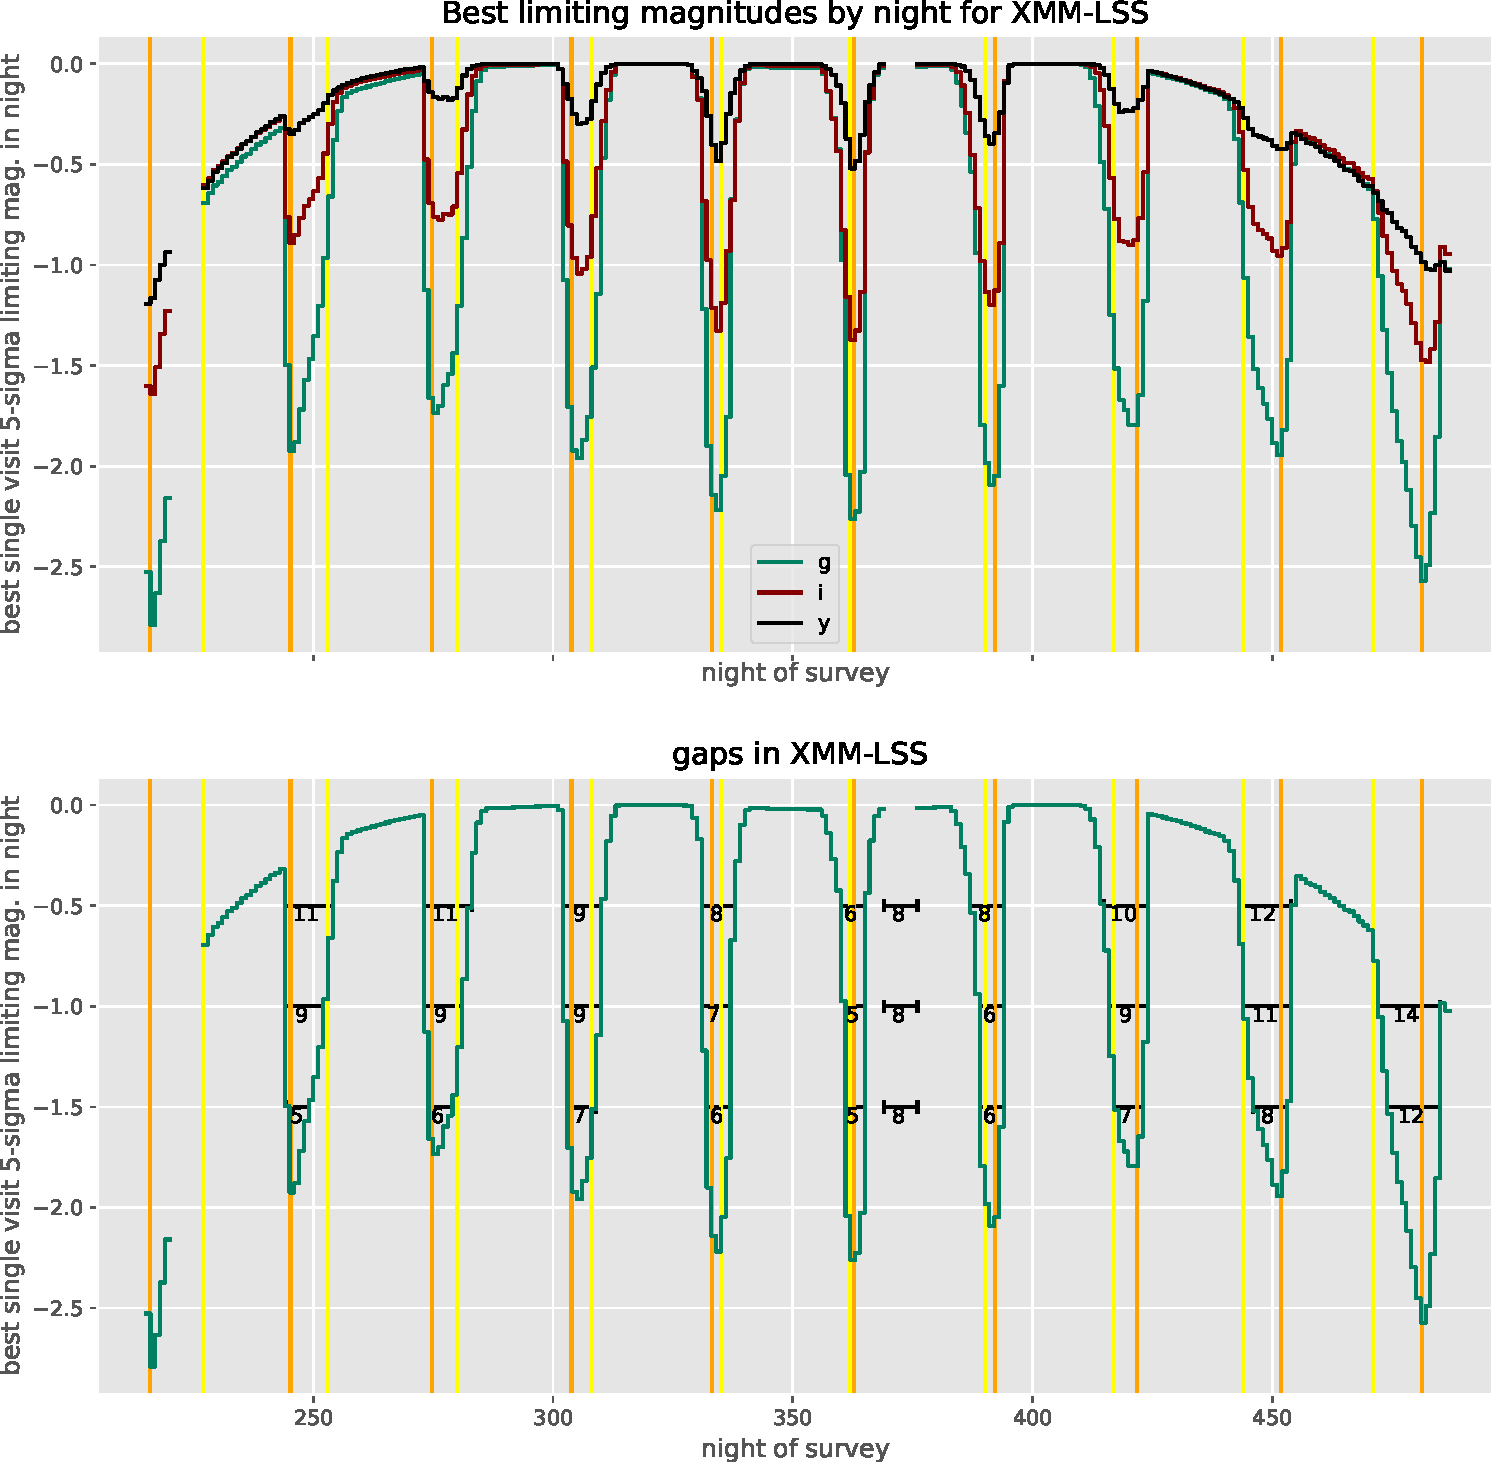
\includegraphics[width=\linewidth]{figures/night_maglim_xmmlss.pdf}
\caption{\label{fig:nightmaglim}
  The top panel shows the $5\sigma$ limiting magnitude of the best visit possible (assuming uniform weather) on each night in the first observing season for the XMM-LSS field, relative to the best possible visit overall, under the same weather and seeing conditions, for three representative filters.
  Other filters are similar, falling between those shown.
  Vertical orange lines show the nights on which the moon is full, and vertical yellow lines show the nights on which the separation between the XMM-LSS field and the moon is at a minimum.
  The lower panel shows the same line for {\it g} band only, and notes the gaps in the cadence forced by varying limiting magnitude, as a function of limiting magnitude (relative to full dark).
}
\end{figure*}

\begin{figure*}
\centering
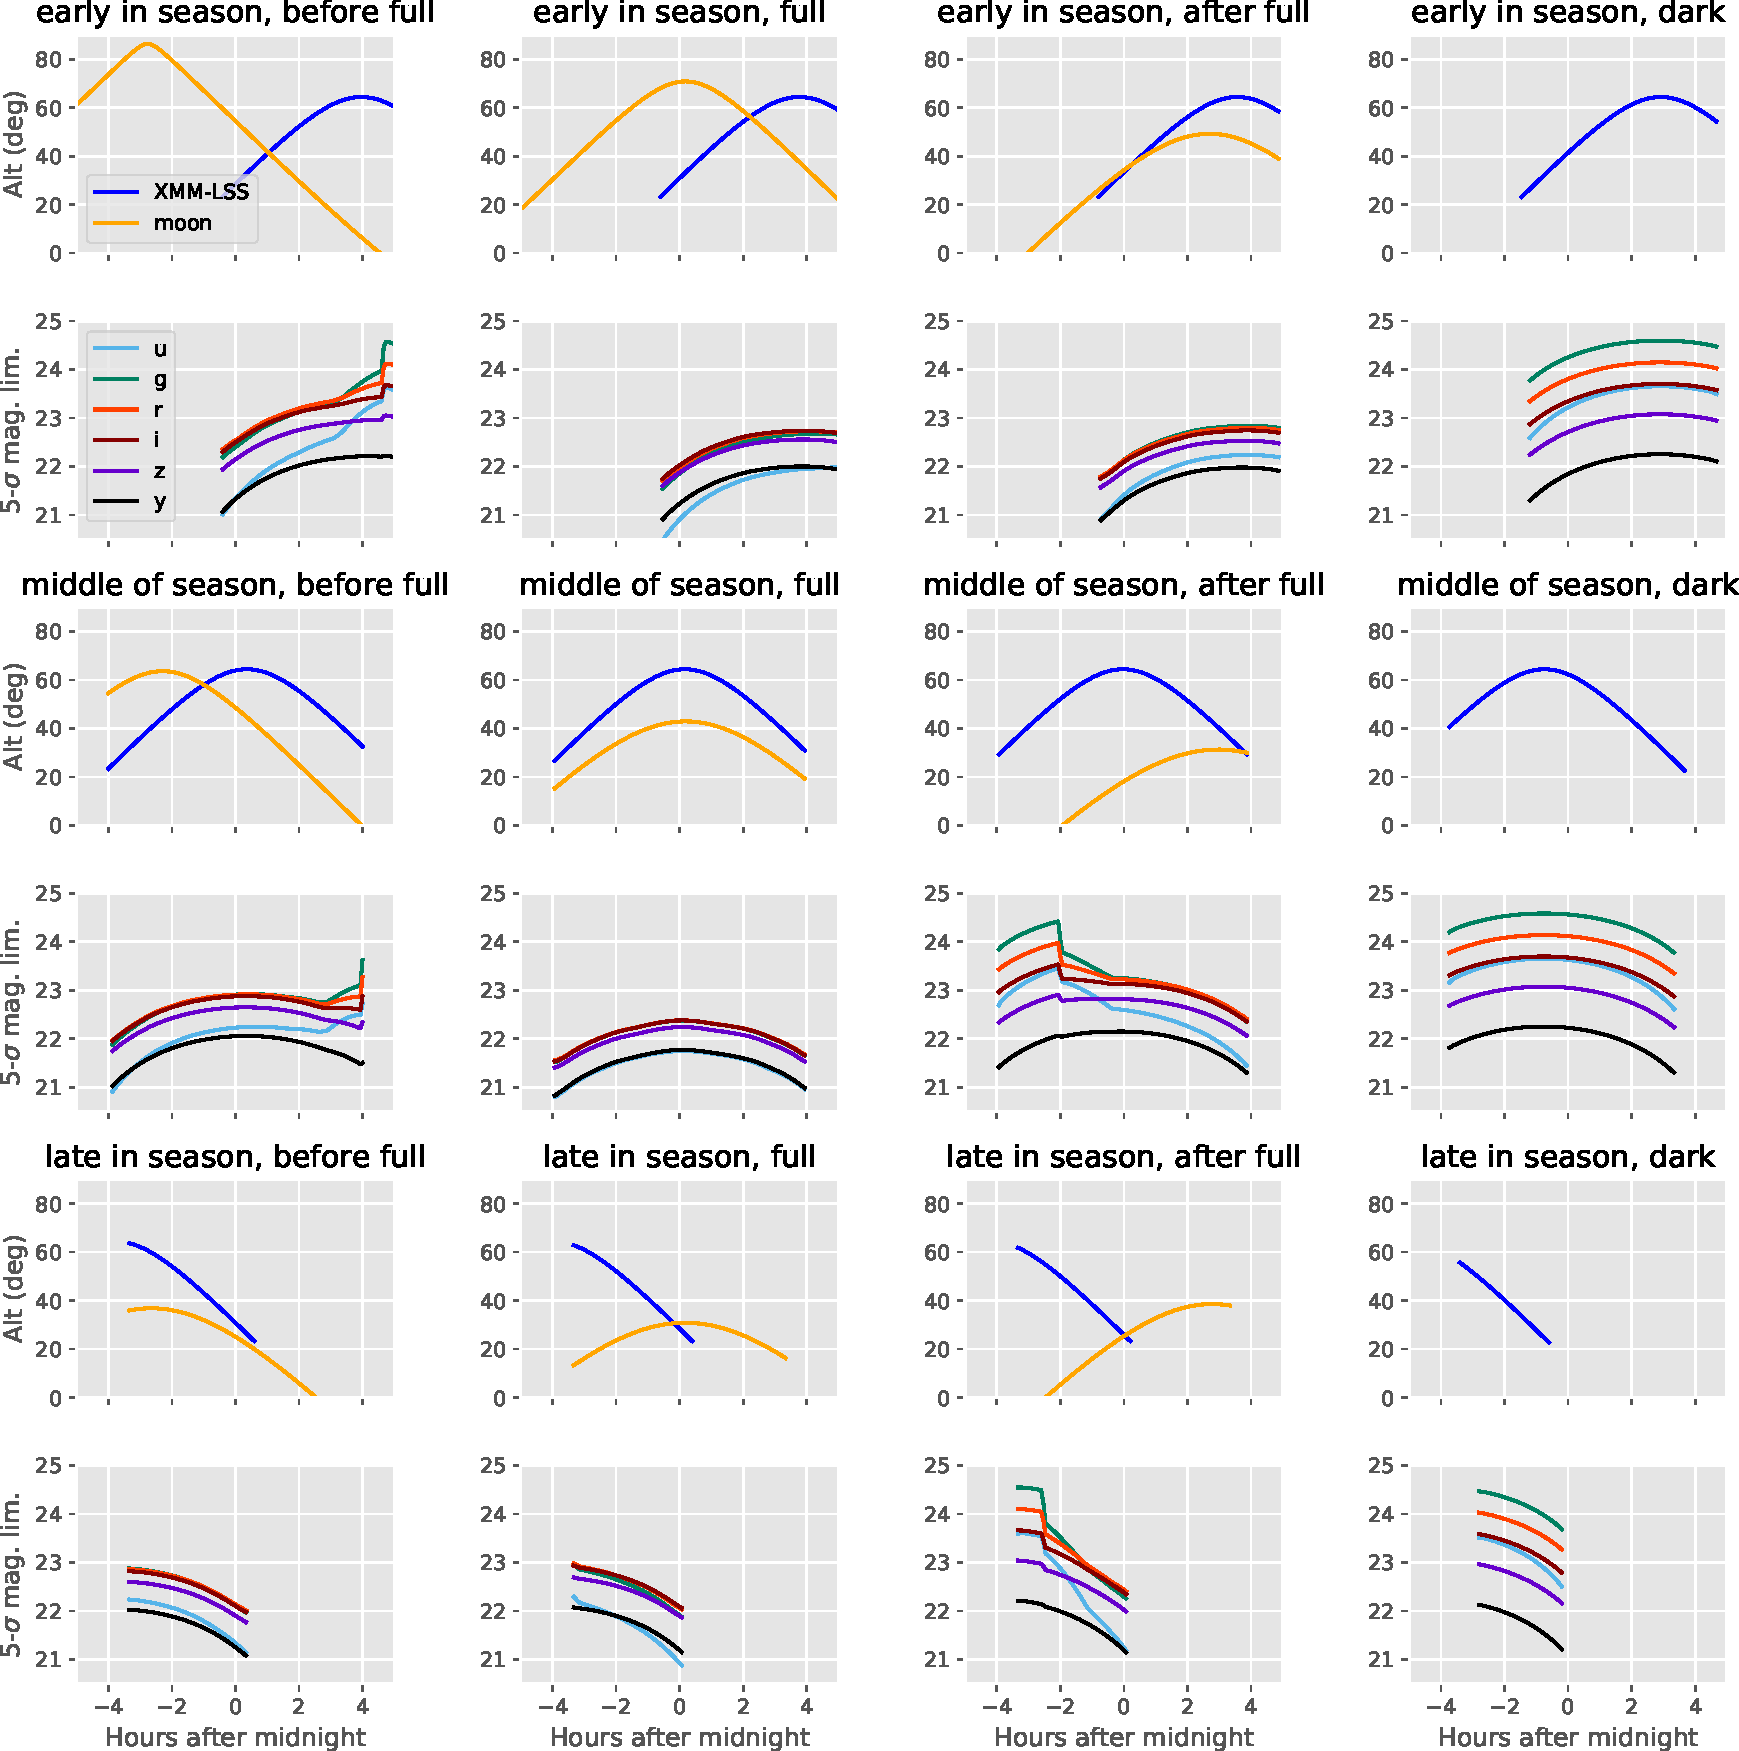
\includegraphics[width=\linewidth]{figures/m5_alt_xmmlss.pdf}
\caption{\label{fig:m5alt}
  These plots show the altitude of the XMM-LSS field (blue) and the moon (gold), and single visit limiting magnitude in different bands in the XMM-LSS field, for a collection of nights during the first season of XMM-LSS observing.
  Each column shows nights at different moon phases: 3 nights before full, full, 3 nights after full, and new.
  Each rows show the curves for a different lunation: the top shows nights around a bright time at the start of the XMM-LSS observing season; the middle, the central bright time in the season; and the bottom, late.
}
\end{figure*}

\section{Bright-time DDF strategy}

Long gaps without detections limit the precision with which light curves can be fit to variable objects.
The LSST DESC explicitly lists the frequency of 7.5 day (or greater) gaps between consecutive visits in the same filter as one of its two primary estimators of desired cadence regularity \citep{scolnic_optimizing_2018}.
The duration of any unavoidable gaps needs to be minimized.
For objects more than two magnitudes brighter than the full dark magnitude limit, no special accommodation of the moon is required: the moon-induced gaps are all shorter than 7.5 days.
For fainter objects, however, the lunar cycle creates gaps in the magnitude time series no matter what the observing cadence is.
To minimize the duration of these gaps, the observing cadence needs to include sequences just before and just after each unavoidable gap.
Otherwise, if these nights are ``off cadence'', the unavoidable gap in the light curves can be (avoidably) lengthened by up to twice the nominal gap between successive sequences (that is, two days for a two day cadence, or four days for a three day cadence).

Figures~\ref{fig:baselinemaglim},~\ref{fig:agnmaglim},~and~\ref{fig:descmaglim} over-plot the limiting magnitudes ``as simulated'' for the first observing season for three reference strategies: the 1.7 baseline and the AGN and DESC proposed strategies \citep{PSTN-051}.
The differences between the uniform weather best visit line (green) and simulated visit (blue) limiting magnitude arises from variations in seeing, and visits taken at times of night that are not optimal.
The gap near MJD 60250 is the result of scheduled downtime.
The baseline starts the season with a short cadence, but the scheduler limits the time spent on DDFs to keep it at the desired fraction of total survey time. This limitation results in long gaps between nights on which the DDFs are visited later in the season. The AGN and DESC strategies reduce the time spent on each DDFs on each night they are visited, and so keep a shorter cadence through the season.

\begin{figure*}
\centering
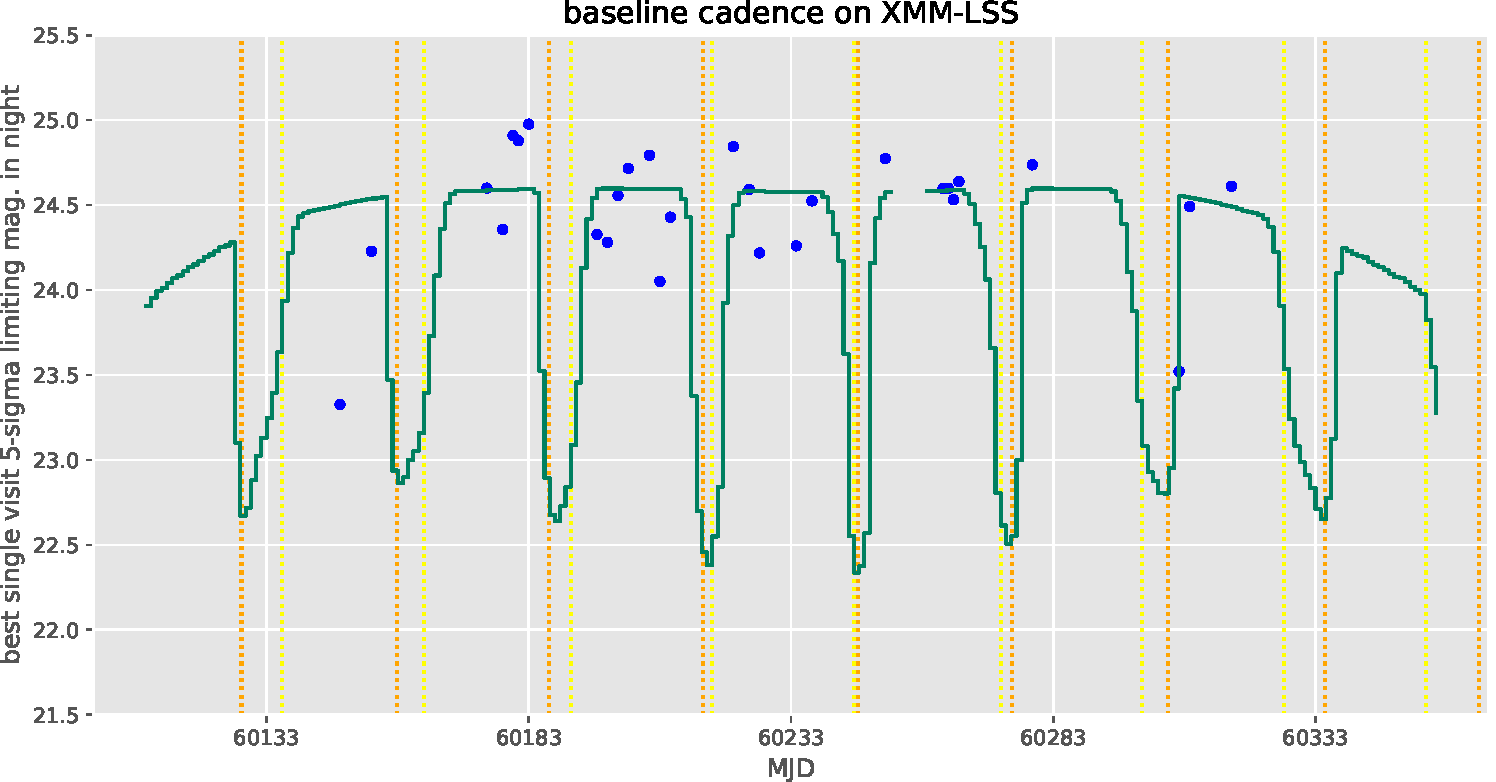
\includegraphics[width=\linewidth]{figures/baseline_nexp2_v1_7_10yrs_xmmlss.pdf}
\caption{\label{fig:baselinemaglim}
  The green curve above shows the single-visit $5\sigma$ limiting magnitude in {\it g} of the best visit possible (assuming uniform weather) on each night in the first observing season for the XMM-LSS field.
  Vertical orange lines show the nights on which the moon is full, and vertical yellow lines show the nights on which the separation between the XMM-LSS field and the moon is at a minimum.
  Blue points show the $5\sigma$ limiting magnitude in {\it g} in the \texttt{baseline\_nexp2\_v1.7\_10yrs} simulation, at the simulated times on nights and seeing from the simulation.
}
\end{figure*}

\begin{figure*}
\centering
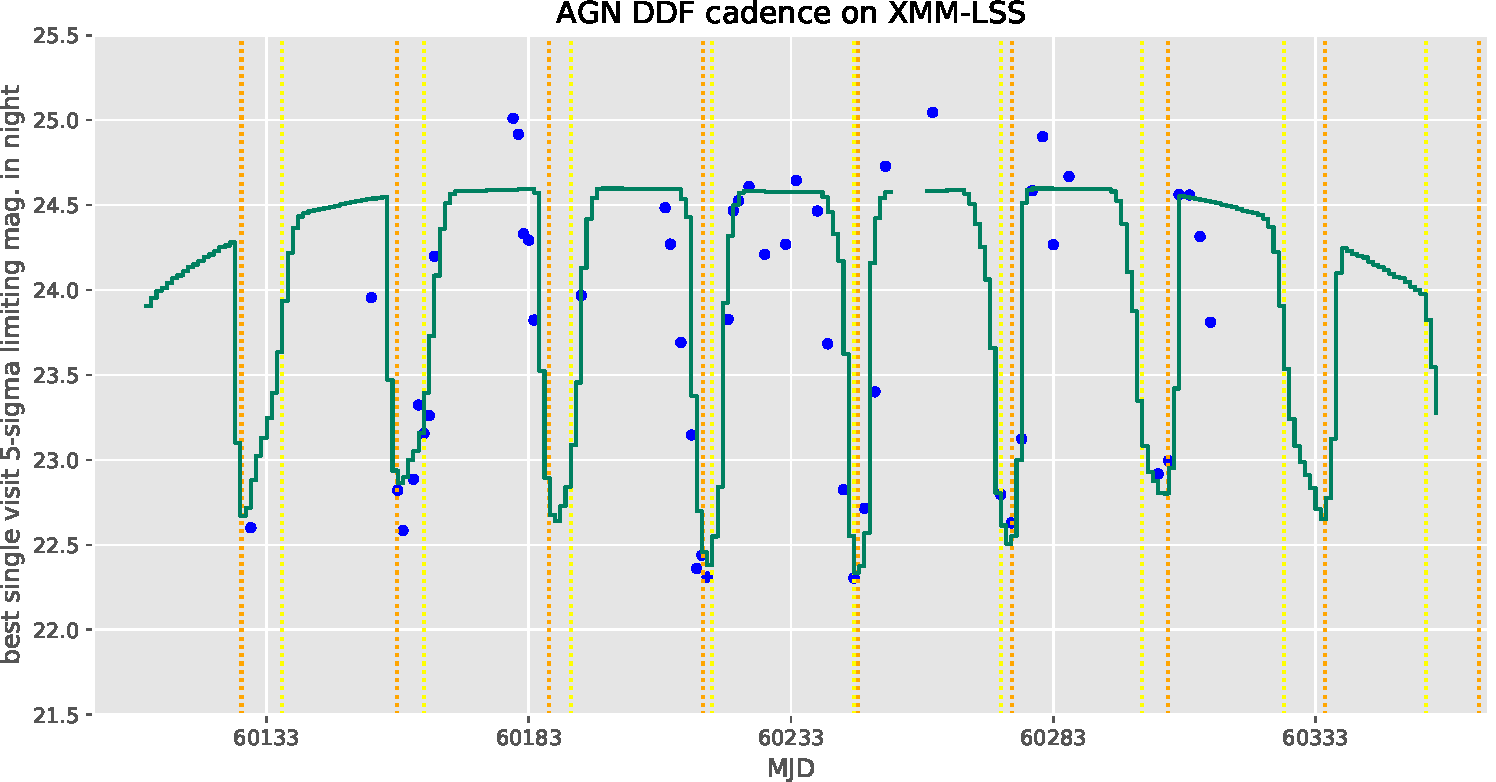
\includegraphics[width=\linewidth]{figures/agnddf_v1_5_10yrs_xmmlss.pdf}
\caption{\label{fig:agnmaglim}
  Markings above represent the same things they do in figure~\ref{fig:baselinemaglim}, except that the blue points represent the \texttt{agnddf\_v1.5\_10yrs} simulation.
}
\end{figure*}

\begin{figure*}
\centering
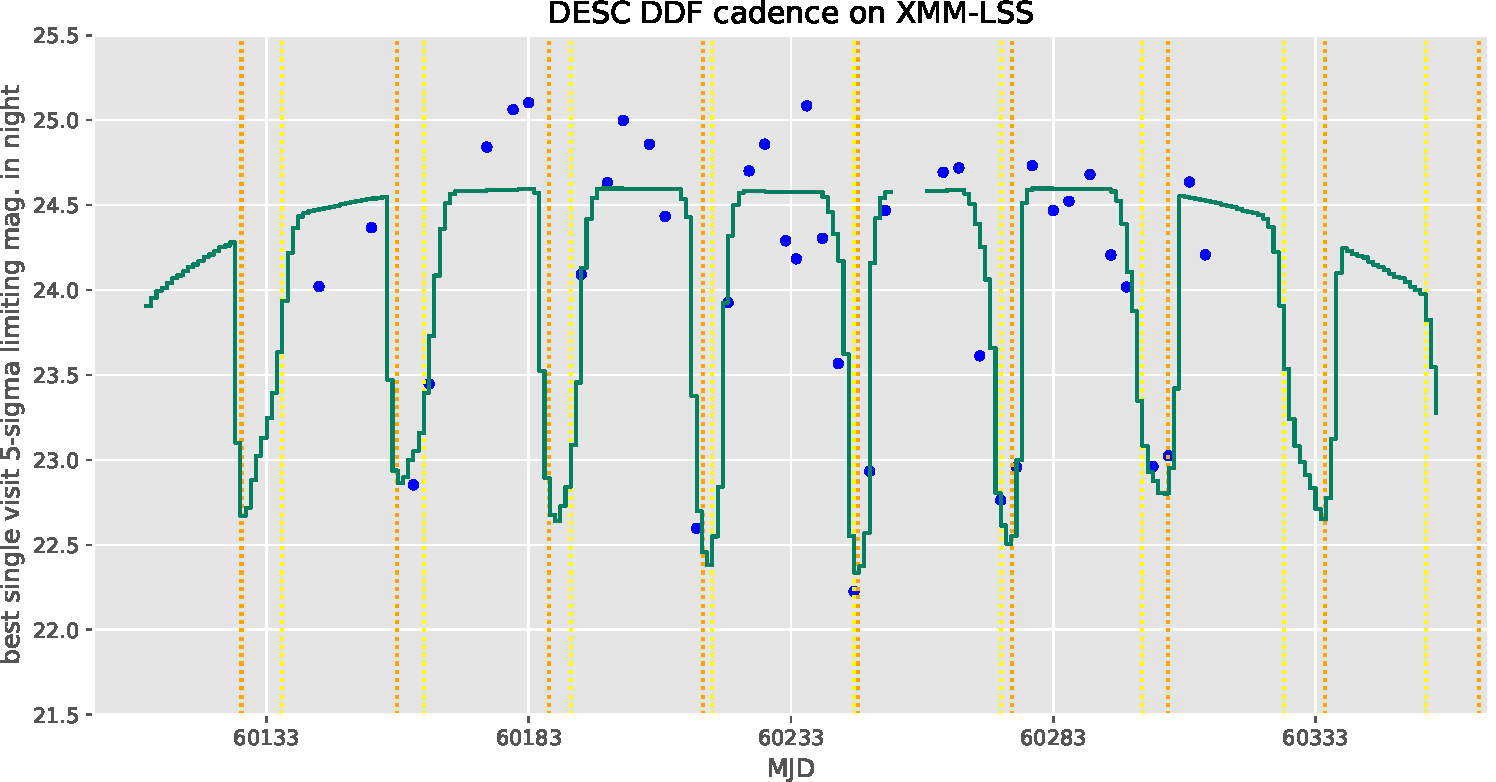
\includegraphics[width=\linewidth]{figures/desc_v1_5_10yrs_xmmlss.pdf}
\caption{\label{fig:descmaglim}
  Markings above represent the same things they do in figure~\ref{fig:baselinemaglim}, except that the blue points represent the \texttt{descddf\_v1.5\_10yrs} simulation.
}
\end{figure*}

Note that the AGN and DDF strategies all include significant numbers of nights on which the single visit limiting magnitude was more than 1.5 magnitudes brighter than full dark, which introduces gaps in the light curves for fainter objects.
Scheduling sequences of exposures on the nights before and after each bright time gap shortens them directly, at the expense of increasing time needed to complete the DDF survey.
This apparently simple strategy raises two questions:
\begin{enumerate}
\item \textbf{What magnitude limit should be used to define the gap?} At the end of bright times early in a field's observing season, the limiting magnitude gradually increases over the course of several nights.
  At the start of bright times late in each season, they gradually drop.
  The precise magnitude cutoff being targeted will determine on which night within each of these sets of nights observing sequences will be scheduled.
  Although this strategy will minimize the gaps for objects brighter than this target, there is the potential to even lengthen the gap for objects just fainter than the cutoff, particularly late in the season, because the new post-gap sequences will not be deep enough to detect them, but they will reset the observing cadence.
\item \textbf{How should the fields be prioritized with respect to each other?} Several DDF fields have highly overlapping seasons, such that the fields are at an observable airmass at roughly the same times. On the ends of nights early in their season, when the moon has set but they are still observable, the last night before the bright time is the same for all of these fields, but the time available on that night is very limited. Similarly, the first dark time after a bright time at the end of their season is at the beginning of the night before the moon as risen, and the time available on that night is similarly limited. A strategy is required to determine which field gets observed during this time. Some approaches include:
  \begin{itemize}
  \item Only apply the additional sequences before and after bright time to one of the fields, and allow the others to occur at their regular cadence, and not necessarily at the optimal time during those nights.
  \item Rank the fields in order of priority, such that the same field always gets the short gaps around bright time.
  \item The prioritization can be randomized or alternated, such that the long gaps are distributed across the fields.
  \item Depending on the duration of the limited dark time, the exposures in a sequence can be split by filter, such that the bluer filters of all fields can be observed in dark time, while those in redder bands can be observed when the moon is up.
  \end{itemize}
\end{enumerate}

\section{Blindly pre-scheduled DDF sequences}

Figures~\ref{fig:prefn0maglim}~and~\ref{fig:prefn2maglim} show the results of simulations that ``pre-schedule'' all DDF nights by applying a regular 2 day or 3 day cadence, supplemented by additional sequences just before and after each bright time to minimize the gaps in light curves for faint objects.
While this strategy does schedule sequences at the edges as intended, it suffers from the significant limitation that it does not accommodate poor weather.
A better approach would be to rerun the pre-scheduler after each night lost to weather, such that missed DDFs can be scheduled immediately thereafter.

\begin{figure*}
\centering
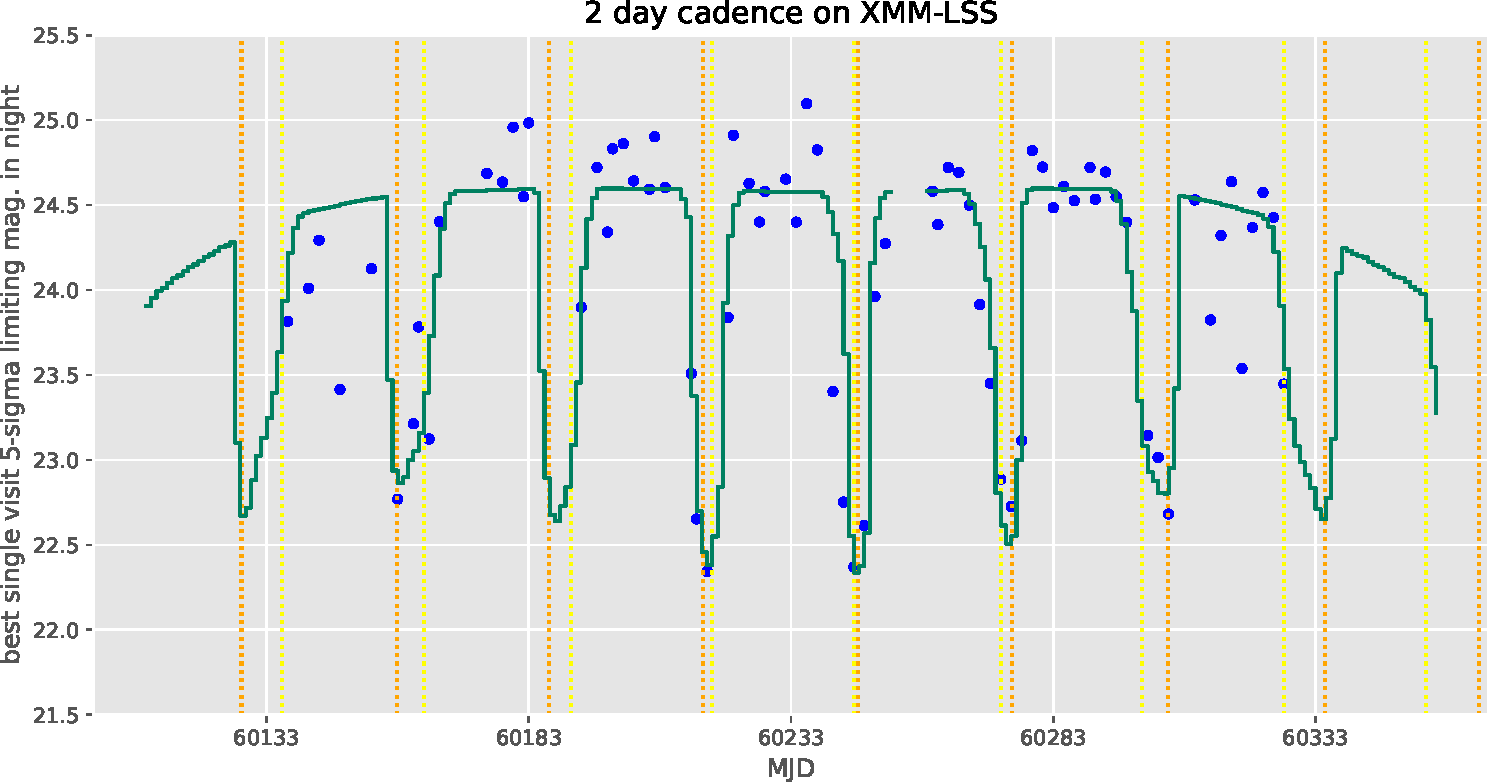
\includegraphics[width=\linewidth]{figures/ddf_pre_fn0_v1_7_10yrs_xmmlss.pdf}
\caption{\label{fig:prefn0maglim}
  Markings above represent the same things they do in figure~\ref{fig:baselinemaglim}, except that the blue points represent the \texttt{ddf\_pre\_fn0\_v1.7\_10yrs} simulation.
}
\end{figure*}

\begin{figure*}
\centering
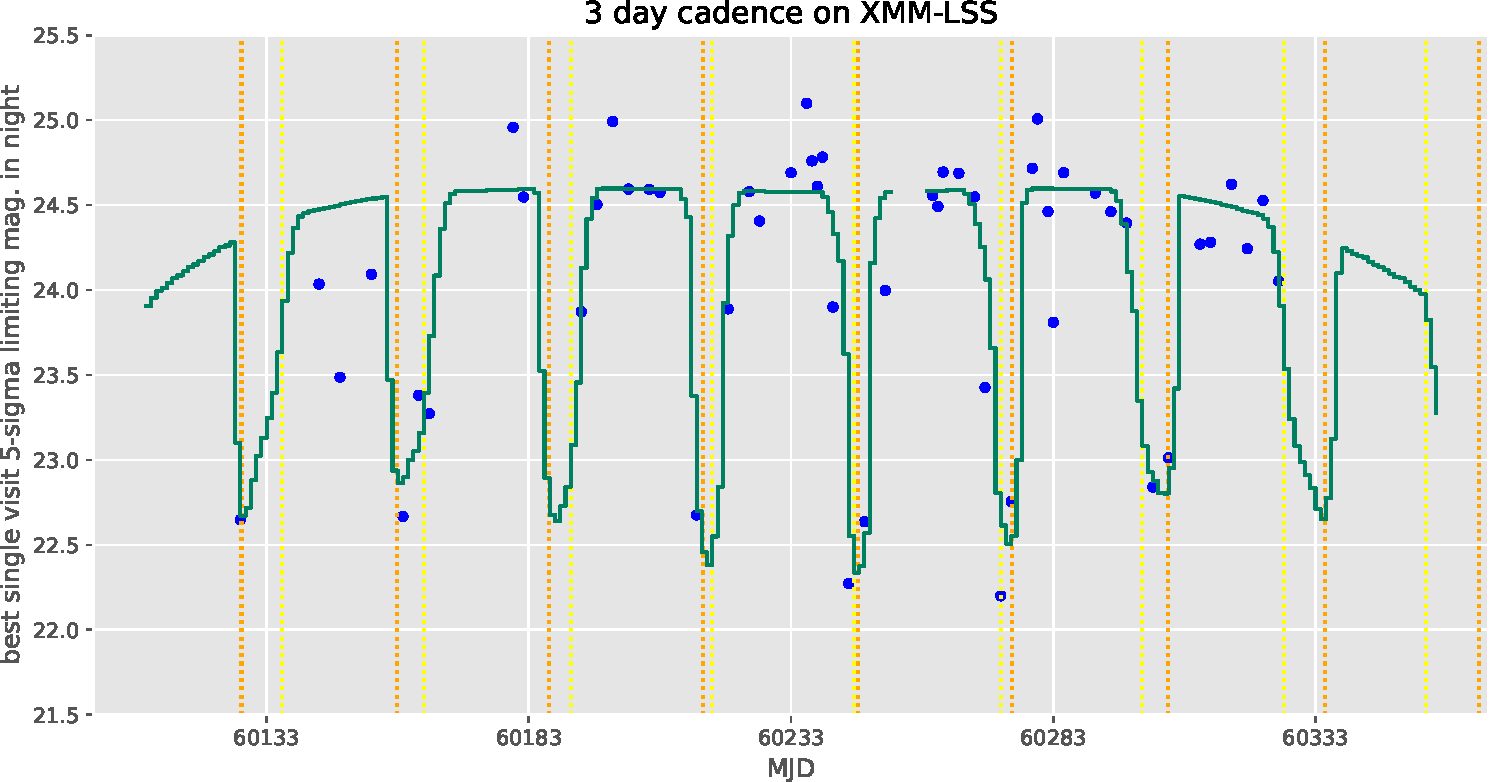
\includegraphics[width=\linewidth]{figures/ddf_pre_fn2_v1_7_10yrs_xmmlss.pdf}
\caption{\label{fig:prefn2maglim}
  Markings above represent the same things they do in figure~\ref{fig:baselinemaglim}, except that the blue points represent the \texttt{ddf\_pre\_fn2\_v1.7\_10yrs} simulation.
}
\end{figure*}

\section{Simulation metrics}


\begin{table}[t]
  \centering
  \begin{tabular}{llrrrrr}
    \hline
         &                   &  nights  &  mean gap &  max gap &  long gaps &  season length \\
   depth & sim &             &           &          &            &                \\
    \hline
20.0 & baseline\_nexp2\_v1.7\_10yrs &         270 &       6.0 &       22 &         71 &            146 \\
     & agnddf\_v1.5\_10yrs &         571 &       3.1 &       19 &         53 &            159 \\
     & descddf\_v1.5\_10yrs &         490 &       3.6 &       11 &         27 &            159 \\
     & 2 day prescheduled &         782 &       2.4 &       11 &         20 &            171 \\
     & 3 day prescheduled &         598 &       3.3 &       12 &         31 &            177 \\
\hline
23.0 & baseline\_nexp2\_v1.7\_10yrs &         270 &       6.0 &       22 &         71 &            146 \\
     & agnddf\_v1.5\_10yrs &         395 &       4.4 &       21 &         71 &            156 \\
     & descddf\_v1.5\_10yrs &         395 &       4.4 &       15 &         58 &            156 \\
     & 2 day prescheduled &         639 &       2.9 &       13 &         49 &            170 \\
     & 3 day prescheduled &         505 &       3.7 &       14 &         58 &            173 \\
\hline
23.5 & baseline\_nexp2\_v1.7\_10yrs &         266 &       6.0 &       22 &         70 &            144 \\
     & agnddf\_v1.5\_10yrs &         303 &       5.2 &       22 &         82 &            144 \\
     & descddf\_v1.5\_10yrs &         353 &       4.8 &       19 &         64 &            154 \\
     & 2 day prescheduled &         537 &       3.3 &       16 &         68 &            163 \\
     & 3 day prescheduled &         428 &       4.4 &       19 &         75 &            171 \\
\hline
24.0 & baseline\_nexp2\_v1.7\_10yrs &         236 &       6.4 &       22 &         66 &            134 \\
     & agnddf\_v1.5\_10yrs &         248 &       6.1 &       23 &         76 &            139 \\
     & descddf\_v1.5\_10yrs &         302 &       5.4 &       20 &         61 &            146 \\
     & 2 day prescheduled &         469 &       3.7 &       18 &         67 &            159 \\
     & 3 day prescheduled &         365 &       5.1 &       20 &         74 &            167 \\
\hline
\end{tabular}
  \caption{
    Simple metrics for the example simulations.
    ``nights'' is the total nights on which XMM-LSS DDF sequences were scheduled.
    ``mean gap'' is the mean gap within seasons.
    ``max gap'' is the mean (over seasons) maximum gap.
    ``long gaps'' is the total number of gaps more than 7.5 days within seasons.
    ``mean season'' is the mean season length.
    Note that these include two partial seasons, one at the beginning and one at the end of the survey, such that the central 9 seasons will be longer than the first and last.
    The season length and mean and max gap columns are in units of nights. 
  }
\label{tab:simplemetrics}
\end{table}

Table~\ref{tab:simplemetrics} shows a collection of simple DDF metrics for the example simulations, cut at several ({\it g}~band) magnitude limits.
The table shows that both pre-scheduled simulations use significantly more nights than any of the feature based schedule (FBS) DDF simulations listed, and also a significantly longer season length.
The different simulations show significantly different number of nights with visits and season lengths.
The baseline has fewer nights, but more visits on each night on which any given DDF is observed, resulting in deeper coadded limiting magnitudes on those nights.
Both the AGN and DESC strategy simulations reduce the number of visits on each night on which the DDFs are observed, but increase the number of nights, resulting in a tighter mean cadence.
The prescheduled simulations both require more nights of observing still, have an even shorter mean cadence (particularly at fainter limiting magnitudes), and longer season lengths; to use the same fraction of survey time, either sequences of visits would need to be shorter still, or the season lengths would need to be truncated.
The hoped for decrease in numbers of long gaps from scheduling DDF sequences carefully at the edges of bright time is not evident, probably because it is more than counterbalanced by the pre-schedulers inability to respond to time lost due to poor weather.

Note that, for a given strategy, decreasing the limiting magnitude can either increase or decrease the total number of long gaps. Decreasing a the limiting magnitude can turn two consecutive stort gaps into a single long one, if the central visit is brighter than the increased limiting magnitude. If, on the other hand, there is a long gap at the end of the season, and the final exposure is brighter than the decreased limiting magnitude, the effect of decreasing the limiting magnitude is to shorten the season and eliminate the final long gap (whose nights are now considered part of the gap between seasons). Also, if two long gaps are separated by a visit with a bright limiting magnitude, increasing the limiting magnitude can merge the two separate long gaps into a single one.

\section{Conclusion and future work}

Although careful scheduling around bright times to minimize moon phase induced gaps in the light curves of faint objects seems important, the initial simple pre-scheduler did not show much improvement, primarily due to the prevalence of gaps due to weather, and the pre-scheduler's fragility with respect to poor weather.
Two strategies are good candidates for improving on these simulations:
\begin{enumerate}
  \item Instead of using a pure pre-scheduler, creating a schedule once at the beginning of the survey and not updating it at all over the next 10 years, rerun the pre-scheduler after each night lost due to weather. This can be refined further by providing the pre-scheduler with upcoming nights forecast to be cloudy so that they can be included in gaps that need to be scheduled around.
  \item Instead of using the pre-scheduler to schedule all DDF sequences, use the pre-scheduler to supplement the current FBS scheduler.
    The advantages of the pre-scheduler are that it can carefully schedule DDFs at the edges of bright time, and optimize when during a given night the DDFs get scheduled.
    The first of these advantages can be achieved by letting the pre-scheduler add nights at the edges of bright times, but have the FBS scheduler schedule other sequences.
    The second of these advantages can be achieved either by using short (one night) FBS scheduler simulations determine whether a DDF should be scheduled on a night, but then having the pre-scheduler optimize the specific time during the night.
    For even better optimization of the time within each night a DDF should be scheduled, a linear-programming optimizer could be used \citep{bellm_zwicky_2019}.
\end{enumerate}


\appendix
% Include all the relevant bib files.
% https://lsst-texmf.lsst.io/lsstdoc.html#bibliographies
\section{References} \label{sec:bib}
\renewcommand{\refname}{} % Suppress default Bibliography section
\bibliography{local,lsst,lsst-dm,refs_ads,refs,books}

% Make sure lsst-texmf/bin/generateAcronyms.py is in your path
\section{Acronyms} \label{sec:acronyms}
\input{acronyms.tex}
% If you want glossary uncomment below -- comment out the two lines above
%\printglossaries

\section{Acknowledgements} \label{sec:acknowledgement}

This manuscript has been authored by Fermi Research Alliance, LLC under Contract No. DE-AC02-07CH11359 with the U.S. Department of Energy, Office of Science, Office of High Energy Physics.

\end{document}
